\subsection{The Equation - Hall Effect}

\begin{equation}
 {\LARGE{\textbf{$V =\frac{Bi}{{ned}}$}}}
 \label{eqn:equation}
\end{equation}


\subsection{Analysis}
Following contains a brief explanation of the variables and the importance of the equation:
\begin{itemize}
\item {\normalsize {The given equation \ref{eqn:equation} has terms \textbf{V} ,\textbf{B} , \textbf{i} ,\textbf{n} ,\textbf{e} and  \textbf{d}.}}

{ Here,}\\
{\textbf{V} represents the voltage across the two plates }\\
{\textbf{B} \  represents the magnetic field between the two plates}\\
{\textbf{i} \  represents the current flowing between the two plates}\\
{\textbf{n} \  represents the density of charge carrier}\\
{\textbf{e} \ represents the electronic charge}\\
{\textbf{d} \ represents the distance between the two plates}
\end{itemize}

If an electric current flows through a conductor in a magnetic field, the magnetic field exerts a transverse force on the moving charge carriers which tends to push them to one side of the conductor. This is most evident in a thin flat conductor as illustrated. A buildup of charge at the sides of the conductors will balance this magnetic influence, producing a measurable voltage between the two sides of the conductor. The presence of this measurable transverse voltage is called the Hall effect after E. H. Hall who discovered it in 1879. \cite{weblink1}

\begin{figure}[h]
	{\begin{center}
		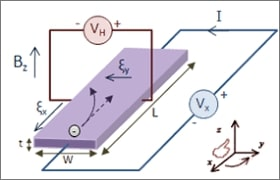
\includegraphics[scale=0.60]{ME20B004.jpg}
	\end{center}}
	\caption{Hall Effect \cite{pic}}
	\label{f1:image}
\end{figure}


\subsection{Applications}
Hall probes are often used as magnetometers, i.e. to measure magnetic fields, or inspect materials (such as tubing or pipelines) using the principles of magnetic flux leakage.
Hall effect devices produce a very low signal level and thus require amplification. While suitable for laboratory instruments, the vacuum tube amplifiers available in the first half of the 20th century were too expensive, power consuming, and unreliable for everyday applications. It was only with the development of the low cost integrated circuit that the Hall effect sensor became suitable for mass application. Many devices now sold as Hall effect sensors in fact contain both the sensor as described above plus a high gain integrated circuit (IC) amplifier in a single package. Recent advances have further added into one package an analog-to-digital converter and I²C (Inter-integrated circuit communication protocol) IC for direct connection to a microcontroller's I/O port.
Hall effect sensors are readily available from a number of different manufacturers, and may be used in various sensors such as rotating speed sensors (bicycle wheels, gear-teeth, automotive speedometers, electronic ignition systems), fluid flow sensors, current sensors, and pressure sensors. Common applications are often found where a robust and contactless switch or potentiometer is required. These include: electric airsoft guns, triggers of electropneumatic paintball guns, go-cart speed controls, smart phones, and some global positioning systems. \cite{weblink2}
